\documentclass[12pt,a4paper]{article}
\usepackage[utf8]{inputenc}
\usepackage[spanish]{babel}
\usepackage{amsmath}
\usepackage{amsfonts}
\usepackage{amssymb}
\usepackage{graphicx}
\usepackage{subfig}
\usepackage{float}
\begin{document}
\title{\bf Financial Practicum Proyect }
\author{Andraž Pirnovar, Jaša Štefan, Laura Carvajal  \\ University of Ljubljana}
\date{November, 15th of 2017}
\maketitle{}
\begin{center}
{\small{\bf Summary}}\end{center}
\begin{quote}
{\small 
\ \ \ \ \ This project presents the numerical results of a problem related to the subject of Operational Research. For the resolution of it, we have worked with the programming programs: Python, R and Matlab. You can find some graphs and tables in addition to a clear description of the problem and the main ideas of the program that we have used.}
\end{quote}
\bigskip 
\section*{Problem description and objective}
Let us consider an annulus A. An annulus is a ring-shaped object, bounded by two concentric circles C and C'. Let us assume that C' is the smaller one. Inside the annulus, there is a set of n points, named Pn, that are uniformly randomly distributed. For these points, we find a convex hull CH(Pn). A convex hull of a set of points X in a Euclidean space (or affine space over the reals) is the smaller convex set that contains X. If we were to have a bounded set X of points on a plane, we could visualize the convex hull as a rubber band stretched around the set X. \medskip 
 
The objective of our assignment is to experimentally analyse the length and the area of CH(Pn). We also have to experimentally analyse the probability that the convex hull CH(Pn) contains the inner border (smaller circumference) of the annulus, C'. 
\pagebreak 

\section*{Hypothesis}
The results should depend on the proportion between the smaller and the bigger circle and also on the number of points inside the annulus.\medskip  
 
Our hypothesis is that the length of the convex hull will increase significantly with the number of points till a certain point and then only marginally with further increase. The size of the radius r will also be a significant factor in the length of the hull, presumably even more so than n, as generated points will be squeezed to the outskirts of the annulus with the radius increase. Similar applies to the area.  \medskip 
 
The probability of the convex hull including the smaller circle, C’, should increase with n and decrease with r. \medskip 
 
The method of point generation should be of some importance. Presumably, if points are generated “truly” uniformly, the probability of inclusion should be higher than with the other method, as there will be more points on the outskirts of the annulus. Therefore, the convex hull from the “true” uniform distribution should be longer and should cover a larger area. Because of a bigger hull, we expect the probability of a smaller circle inclusion to be higher when points are distributed “truly” uniformly. 
 
\section*{Theoretical framework}
For the resolution of our problem we will use a Convex hull algorithm, in particular the Gift Wrapping algorithm of Jarvi's March. \medskip

To give theoretical support to our problem we will remember this algorithm:
A convex hull is the shape that completely encloses a set of points with the least number of perimeter nodes.
There are two main properties of convex hulls that should be explored, that all of the points in the final polygon must be convex, and the most extreme point on any axis is part of the convex shell. \medskip

The first phase of the algorithm is to identify the minimum point on some axis. The $ y-axis $ is a good candidate, as the angles for all other points in the set range from $90^{\circ}$  to $270^ {\circ}$ , which facilitates sorting. This makes identifying the point with the minimum angle, relative to the current point, significantly easier.Starting with the minimal point, already known to be in the final perimeter, the algorithm scans all the points in the set, computes their angle, and stores the most angularly minimal point. Because the initial order of the set is arbitrary, it is necessary to scan all nodes in the set except for the current point. Sorting by angle is not useful, because the angles change as the algorithm progresses from point to point. The point found from the process described above will be the next point in the convex hull, in the clockwise direction. If you relate this to the physical example using the rubber band stretched around the set X it is evident that as you put the rubber around the set, the first pin that touches the string will be the one with the least relative angle.\medskip

Once the main algorithm on which our project is based is presented, we turn to the description of procedure and resolution tools.

\section*{Methodology}
Most of the programing work has been done in Python and Matlab, with some graphics and analysis done in R. Most of the project specific code has been written by us, with the help of numpy and scipy packages and predefined functions. \medskip

Regarding the generation of data n, we took 16 different values: $$n= 3,4,5,6,7,8,9,10,15,20,30,40,50,100,200,500$$
And we use two methods for point generation:
\begin{enumerate}
 \item The first one distribute the points uniformly over the area of the annulus, using a probability transformation of uniformly distributed polar coordinates parameter.
 \item The other also uses uniformly distributed parameters of polar coordinates, but without the transformation, so the points are not uniformly distributed over the annulus.
 \end{enumerate} 

As is known, wee need to experimentally analyse the length, the area of CH(Pn), and also the probability that the convex hull CH(Pn) contains the inner border.
At smaller values, the differences in length, area and probability should be more noticeable with small increases in n than at higher.\medskip

 
As we have to analyse the data with respect to radius r of the smaller circle C’ and number of points n, we decided it would be best if we measure the radius relatively to the radius of the bigger circle. 
 
So we set the bigger radius to 1 and took 101 smaller radiuses, from $0\to 1$. This represents $1\%$ increase of the smaller radius, relative to the bigger one, for which we calculate all of the required properties. \medskip

\begin{figure}[H]
 \centering
  {
   \label{f:graph1}
    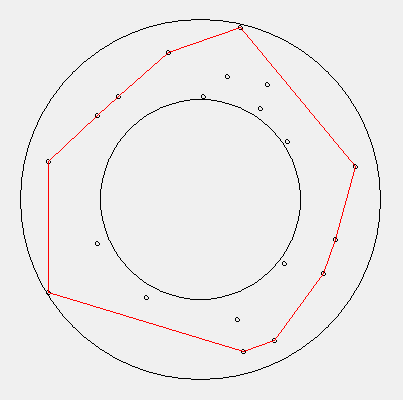
\includegraphics[width=0.3 \textwidth]{convex_hull1.png}} \hspace{25mm}
  {
   \label{f:graph2}
    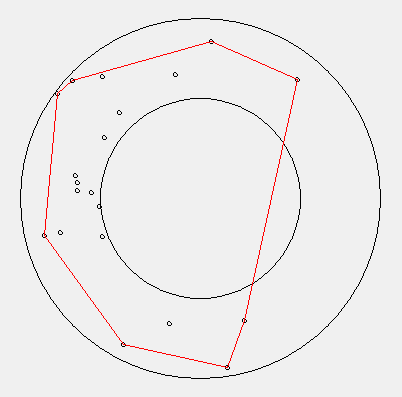
\includegraphics[width=0.3  \textwidth]{convex_hull2.png}}
 \caption{Example of how our convex hull algorithm works. In this case the set have 20 points.}
 \label{f:graphs}
\end{figure}

For each combination of r, n and generating method, we did 4000 repetitions, each time with a new set of randomly generated points. For every combination, we calculated mean length, mean area and the number of times the smaller circle C’ was included inside the convex hull. From this, we calculated the experimental probability of the convex hull containing the inner circle. \medskip
 
Data is saved to a csv, so that it is easy to import into R and make 2D-graphs and 3D-graphs for show and compare better the results.

\section*{Record of results}

We present the results through graphs made with R. 
\begin{itemize}
\item \emph{Length of the convex hull:}

\begin{figure}[H]
 \centering
  \subfloat[With naive distribution]{
   \label{f:length1}
    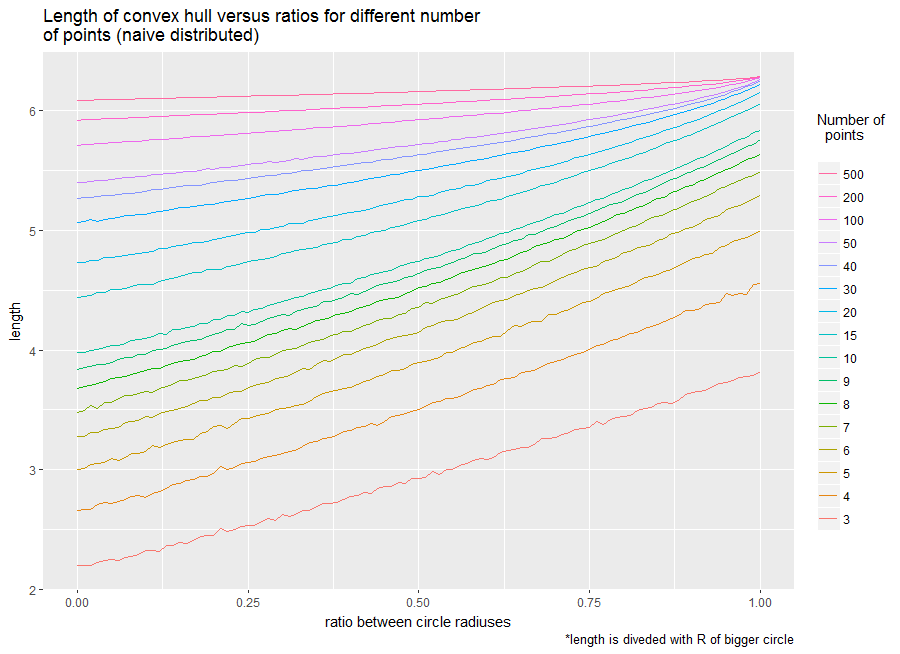
\includegraphics[width=0.5 \textwidth]{length_naive.png}}
  \subfloat[With polar distribution]{
   \label{f:length2}
    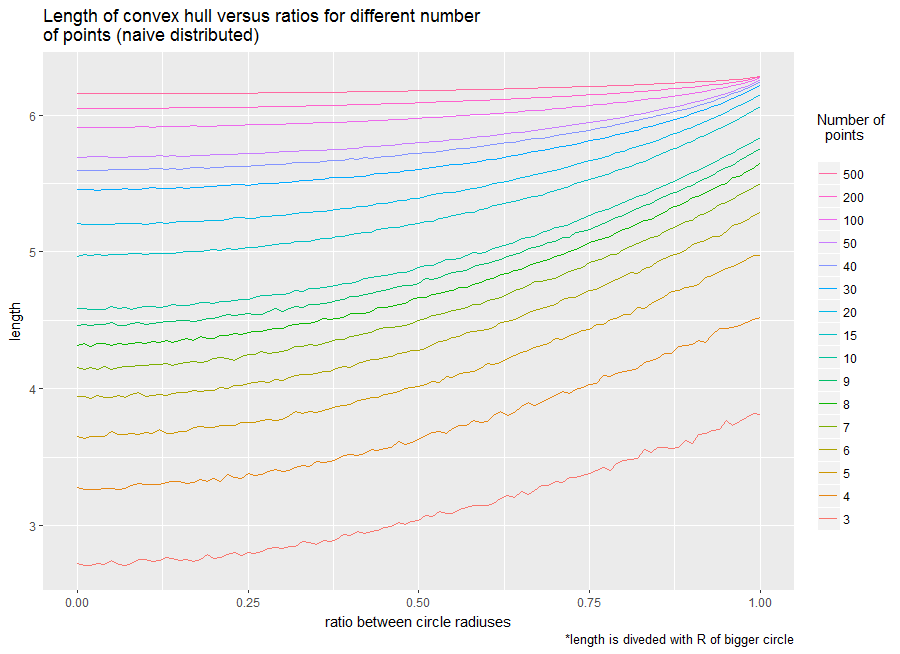
\includegraphics[width=0.5 \textwidth]{length_polar.png}}
 \caption{Graphs with the results obtained when we calculate the convex hull length.}
 \label{f:results_length}
\end{figure}

In this figure(2) we present the resulting data of calculate the length doing 4000 repetition for each combination of r,n. \\
 In the left, figure 2 (a) there is the representation of the results taken the set of points with naive distribution. Therefore in the rigth, figure 2 (b) there ir the representation of the results taken the set of points with the polar distribution. \\
 \\
We can see, in first view that the length of the convex hull increase significantly,as we suspected.

In order to reach a more precise conclusion and be able to analyze the data, we will superimpose the graphs.
\begin{figure}[hbtp]
\centering
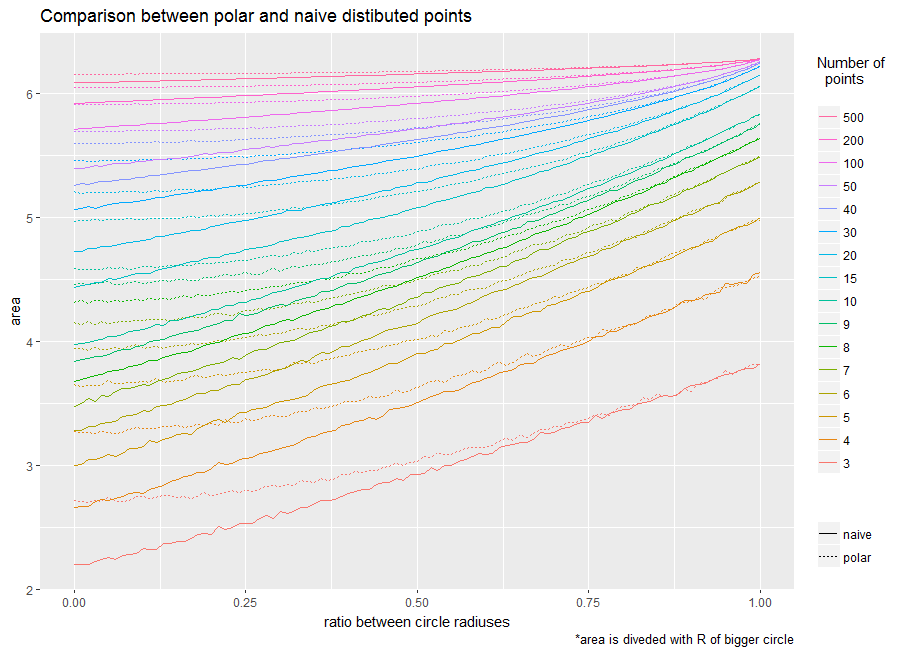
\includegraphics[scale=0.35]{length_comparison.png}
\caption{Graph to compare the results of the length by the two distributions.}
\end{figure}

A continuous line is represented by the data with naive distribution and with discontinuous lines the data with polar distribution.\\
\\
Now, we can see easily that our hypotheses were true. The length of the convex hull increase significantly with the number of points till a certain point and then only marginally with further increase. The size of the radius r will also be a significant factor in the length of the hull, presumably even more so than n, as generated points will be squeezed to the outskirts of the annulus with the radius increase. \\
And also as expected the convex hull resulting from the data with polar distribution have greater length.\pagebreak 

\item \emph{Area of the convex hull:}


\begin{figure}[H]
 \centering
  \subfloat[With naive distribution.]{
   \label{f:area1}
    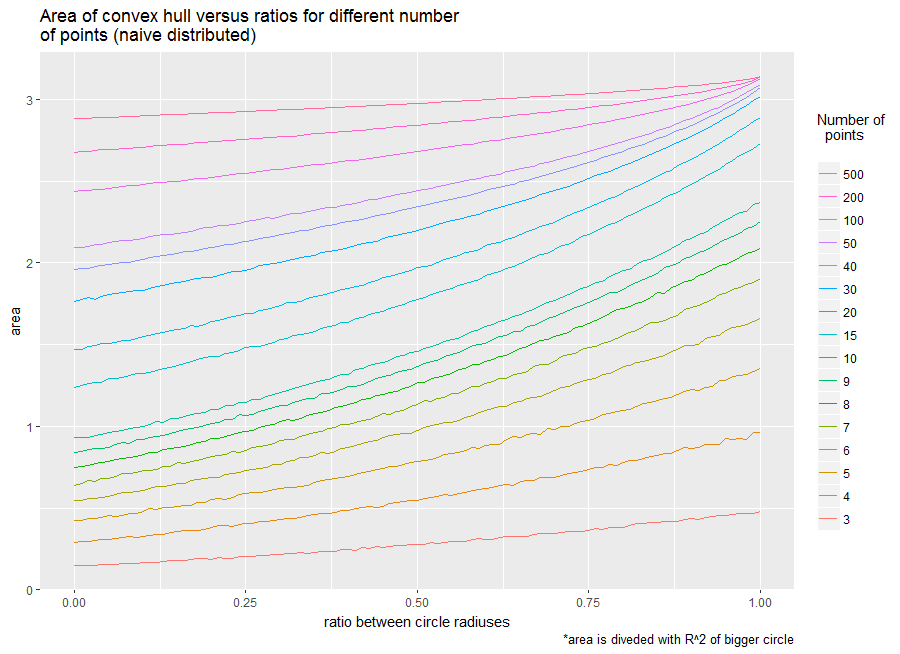
\includegraphics[width=0.5 \textwidth]{area_naive.png}} 
  \subfloat[With polar distribution]{
   \label{f:area2}
    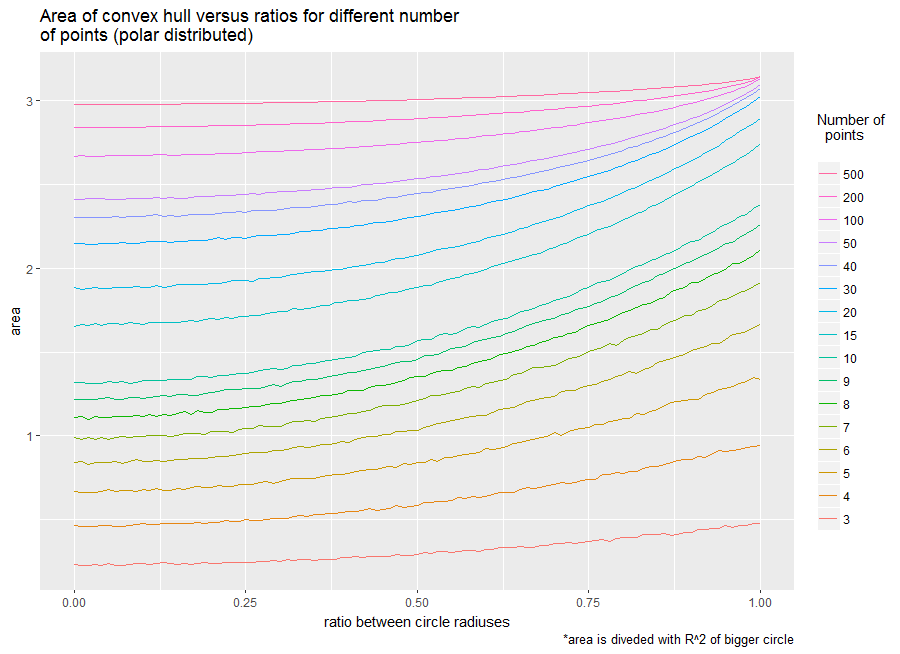
\includegraphics[width=0.5  \textwidth]{area_polar.png}}
 \caption{Graphs with the results obtained when we calculate the convex hull area.}
 \label{f:results_area}
\end{figure}
In the same way, being in the figure(3), the left is the representation of the results taken the set of points with naive distribution. And in the rigth, the representation of the results taken the set of points with the polar distribution. \\ 
 
Besides, the area increase significantly with the number of points and the radius r be more significant factor even than n. 

Let us superimpose the graphs to see the comparison:
\begin{figure}[hbtp]
\centering
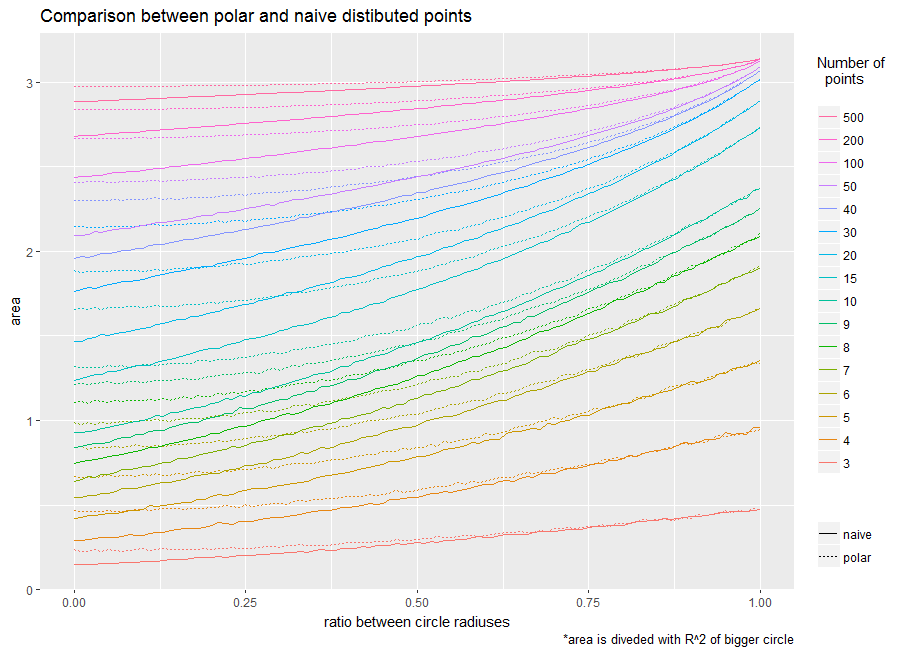
\includegraphics[scale=0.35]{area_comparison.png}
\caption{Graph to compare the results of the area by the two distributions.}
\end{figure}

The continuous line is represented by the data with naive distribution and with discontinuous lines the data with polar distribution.\\
It happens exactly the same as with the length, with the polar distribution the convex hull wraps up more area.


\item \emph{Probability of the convex hull contains the small circunference:}
\begin{figure}[H]
 \centering
  \subfloat[With naive distribution.]{
   \label{f:prob1}
    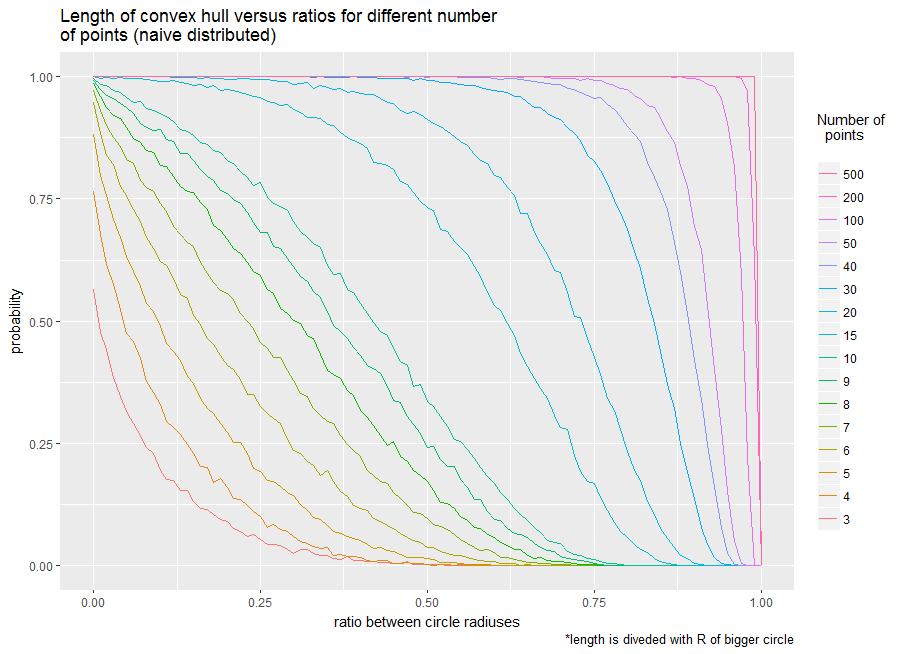
\includegraphics[width=0.5 \textwidth]{probability_naive_new.png}} 
  \subfloat[With polar distribution.]{
   \label{f:prob2}
    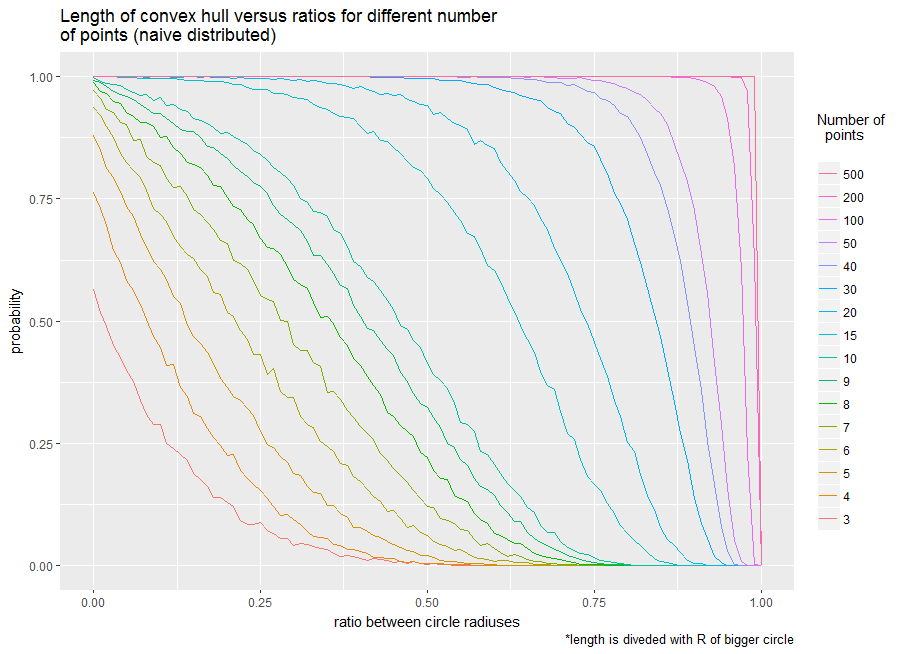
\includegraphics[width=0.5  \textwidth]{probability_polar_new.png}}
 \caption{Graphs with the results obtained when we calculate the probability of the convex hull contains the small circunference C'.}
 \label{f:results_prob}
\end{figure}

We can see that the probability that the convex hull including the smaller circle (C') increase with n and decrease with r in bouth cases, what is quite intuitive.

As in the previous cases, the figure at the left represent the results with the naive distribution, and at the rigth we have the polar distribution. 

Now we going to observe the comparison of both distributions

\begin{figure}[hbtp]
\centering
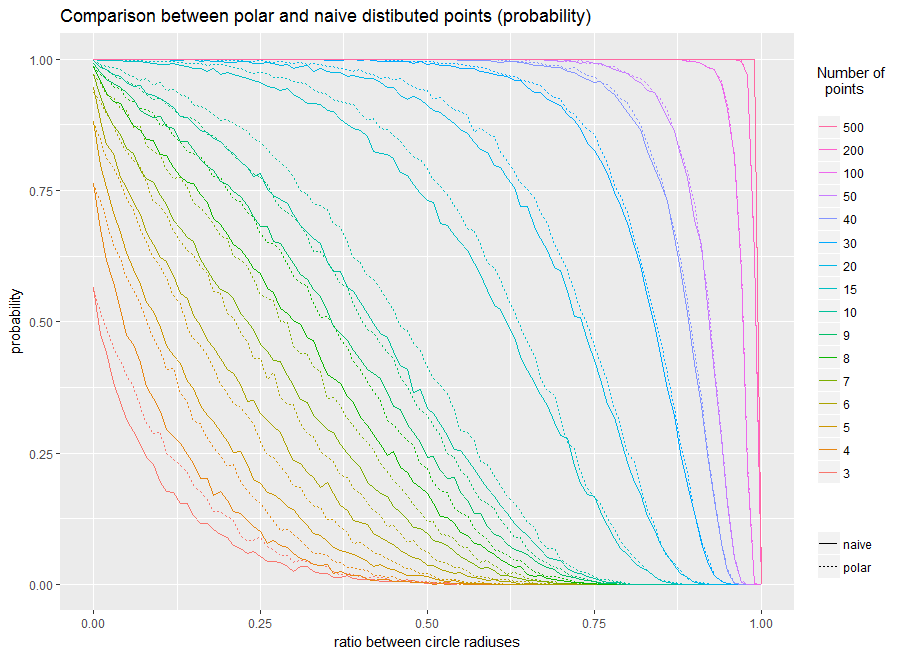
\includegraphics[scale=0.35]{probability_comparison_new.png}
\caption{Graph to compare the results of the probability by the two distributions.}
\end{figure}

With the same ratio of radius the probability results with the polar distributions are more highers. And this have sens because if points are generated “truly” uniformly, the probability of inclusion should be higher than with the other method. 

\end{itemize}
With this section we have finished contrasting all our hypotheses. To finish and  complete the analysis we have added two 3D-graphs with which the results are much better visualized globally.
\begin{figure}[H]
 \centering
  \subfloat[With naive distribution.]{
   \label{f:prob1}
    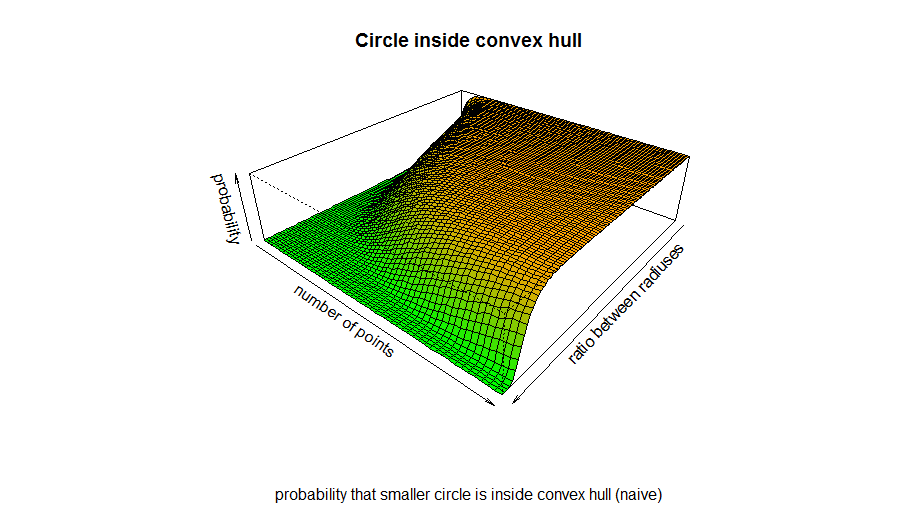
\includegraphics[width=0.5 \textwidth]{3D_naive_new.png}}
  \subfloat[With polar distribution.]{
   \label{f:prob2}
    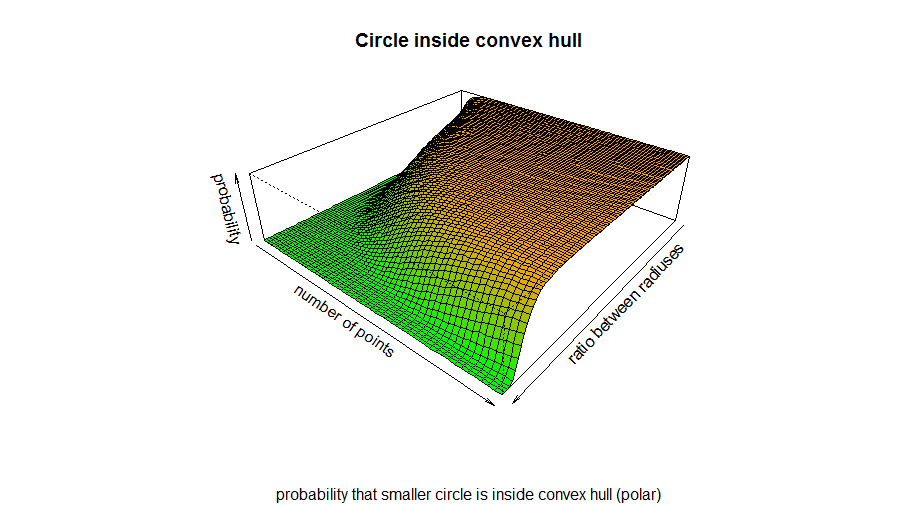
\includegraphics[width=0.5  \textwidth]{3D_polar_new.png}}
 \caption{Graphs 3D with the results obtained}
 \label{f:results_prob}
\end{figure}


\section*{Bibliography}
\begin{enumerate}
\item Cormen, Thomas H.; Leiserson, Charles E.; Rivest, Ronald L.; Stein, Clifford (2001) [1990]. "33.3: Finding the convex hull". Introduction to Algorithms (2nd ed.). MIT Press and McGraw-Hill. pp. 955–956. ISBN 0-262-03293-7.

\item Jarvis, R. A. (1973). "On the identification of the convex hull of a finite set of points in the plane". Information Processing Letters. 2: 18–21. doi:10.1016/0020-0190(73)90020-3.
\end{enumerate}




\end{document}